\documentclass[12pt]{article}

\usepackage{rotating}		% Use sidewaystable command
\usepackage{pdflscape}		% Produce landscape pages in a (mainly) portrait document
\usepackage{float}			% Added this package to place things right where I want them!
\usepackage{mathtools}		% Added this package in order to use shortintertext command
\usepackage{amsmath}
\usepackage{amssymb}
\usepackage{geometry}
\usepackage{graphicx}
\usepackage{tikz}
\usepackage{epstopdf}
\usepackage{caption}
\usepackage{subcaption}
\usepackage{hyperref}

\geometry{letterpaper,tmargin=1in,bmargin=1in,lmargin=1in,rmargin=1in}
\hypersetup{
colorlinks,linkcolor=black,citecolor=violet,urlcolor=blue
}

\allowdisplaybreaks			% Allows equations to be split across multiple pages

\begin{document}

\title{Design 2 Kick-off Report}
\author{Smart Vibes}
\date{January 23, 2017}
\maketitle

\newpage
\tableofcontents

\newpage
\section{A Look Back}
Last semester in Design 1, Smart Vibes set out to design a sensor that can monitor vibrations in the ground for Smart Structures, a global leader in wireless embedded data collector solutions. The sensor will be deployed in construction sites to monitor the stress on buildings caused by piledriving activity and other machinery vibrations. Smart Vibes was able to get together a bill of materials, system level design report, and a project schedule in order to build the vibration sensor this semester.

\section{Project Timeline}
The project timeline in Figure \ref{fig:gantt_chart} shows three milestones Smart Vibes will tackle before reaching the final milestone of building the final prototype. The first milestone comes right after successfully interfacing the accelerometer and geophone with the Adafruit Feather microcontroller; this also means getting the data to write to the SD card and sync to the cloud. The second milestone will be reached immediately after running the sensor strictly off of the lithium-ion battery and recharging the battery with solar power. The third milestone will come when the sensor is placed in its housing and is able to perform most, if not all, of its functions and yield accurate and reliable results.

\begin{figure}[H]
    \centering
    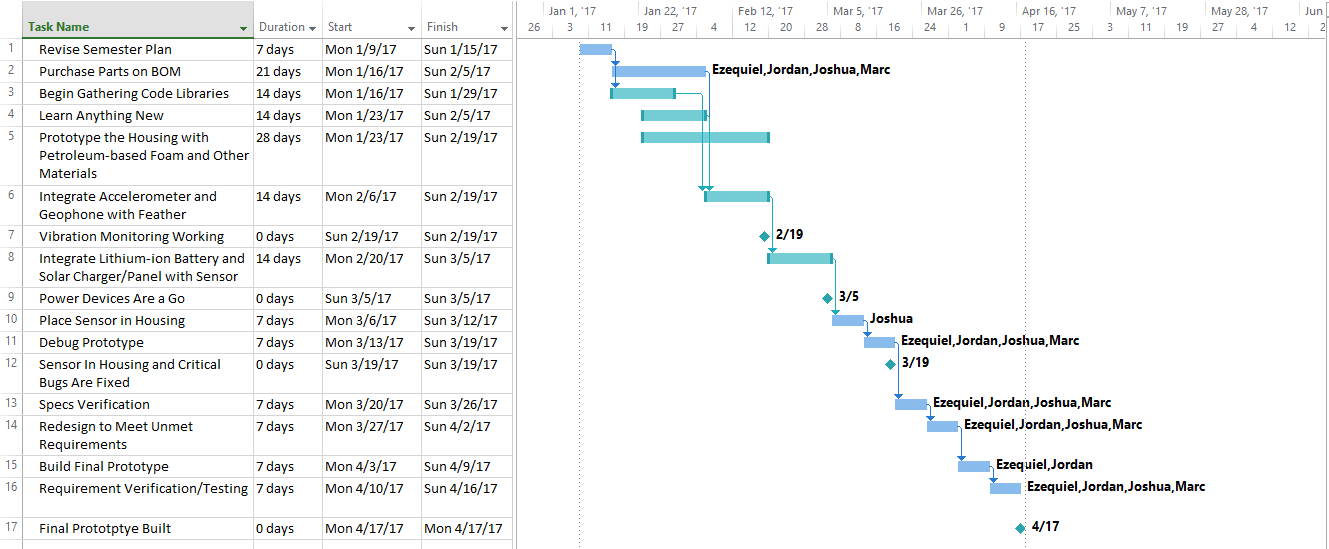
\includegraphics[width=1.3\textwidth, angle=90]{src/gantt_chart.png}
    \caption{Project schedule for Design 2 course.}
    \label{fig:gantt_chart}
\end{figure}

\section{What's Next?}
\textbf{Software Development}
\begin{itemize}
\item Going through different libraries of data
\item Understanding how we can develop software to communicate efficiently with other components in the system
\item Creating a list of objectives to accomplish in software development
\end{itemize}

\noindent \textbf{Hardware Assessment}
\begin{itemize}
\item Understanding how the hardware communicates to one another
\item Refining the enclosure
\item Material Analysis
\item Stress Testing
\item Battery Efficiency
\end{itemize}

\section{Bill of Materials}
The following list includes standard ``off the shelf'' items that we will be incorporating into our design. All items are relatively inexpensive, and are expected to perform adequately under a range of environments.

\begin{itemize}
\item Accelerometer
\item Adafruit Feather Microcontroller
\item MicroSD Card Board
\item 16GB MicroSD Card
\item 6600 mAh 3.7V Battery
\item Enclosure material
\item Solar Panel
\item USB/DC/Solar Lithium Ion/Polymer charger
\item Geophone
\item Coin Cell Battery
\end{itemize}

\section{Work Distribution}

Due to the unfortunate departure of one of our group members, each person will have a few more responsibilities. As it stands at the moment, the distribution of work in Smart Vibes is as follows:\\

\noindent \textbf{Joshua Watkins} - \textit{Mechanical/Design} - Responsibilities include designing an enclosure for the sensors that will maximize the sensor's capabilities while minimizing cost.\\

\noindent \textbf{Marc-Edwin Rigaud} - \textit{Programming} - Responsibility is to program the microcontroller, and arrange website and cloud-based services.\\

\noindent \textbf{Jordan Faison} - \textit{Electrical/Design/Programming} - Responsibilities will be assisting in design from an electrical aspect, as well as software development.\\

\noindent \textbf{Ezequiel Juarez G.} - \textit{Electrical/Programming} - Responsibilities include assembling the vibration sensor system using all of the electronics at our disposal and aiding with the programming/debugging of software.


\end{document}